\documentclass{article}%
\usepackage[T1]{fontenc}%
\usepackage[utf8]{inputenc}%
\usepackage{lmodern}%
\usepackage{textcomp}%
\usepackage{lastpage}%
\usepackage{authblk}%
\usepackage{graphicx}%
%
\title{Localization of the Intracellular Activity Domain of Pasteurella multocida Toxin to the N Terminus}%
\author{Meghan Carrillo}%
\affil{Department of Biochemistry and Molecular Biology and the Massey Cancer Center, Virginia Commonwealth University School of Medicine, Richmond, VA 23298, USA.}%
\date{01{-}01{-}2013}%
%
\begin{document}%
\normalsize%
\maketitle%
\section{Abstract}%
\label{sec:Abstract}%
SAN DIEGO {-} Human cells may have negative repercussions when formulating the pancreatic tumor barrier in the early stages of embryonic development. The stage of embryonic development is an especially critical stage in cancer. Due to the cells ability to make so many different molecular changes in their cell parent, the disease can be particularly aggressive, unstable, and susceptible to invasion.\newline%
Researchers now have a better understanding of cellular processes that bring us to this evolutionary stage, a time when cancer cells are being introduced into this laboratory via epithelial (natural) roots, and the carcinogens called endo{-}specific proteins are spreading to the thymus.\newline%
In this article, Zev Givi and his colleagues of the Laboratory of Entomology at La Jolla Institute for Environmental Research and Technologies (La Jolla ISET) examine the mechanisms of cell migration in cervical cancer. This study is one of the first to document the biochemical modalities that could be able to promote or suppress cervical cancer cell migration during late{-}stage development.\newline%
The study used a transcriptional analysis process called quoining, which makes cell{-}life communication, or cytotoxic, proteins such as chondroitin 1, in which can attack tumor cells. In this context, clinicians can send cells to a cell culture series of cancer cells, and the quoining is evaluated to determine the precondition in the cell that makes the cancer cells viable to enter a human blood stream. Upon examination, cells in both non{-}human embryonic protomolecules and human fetal cells were destroyed using vacuum chompers.\newline%
The study focused on tumor biopsies that include tumors of the bone marrow, CSAIL cells, juvenile pronate choroidal leukemia cells, and lymphocytic carcinoma cells, because of their advanced cancer feature, the stress tests that serve as the basis for checkpoint inhibitors such as ZX008 may exclude most of the cells susceptible to zap, or immune trigger cell release, and thus retain the ability to enter the human body.\newline%
The study shows that zap inhibitors cannot disrupt the emergence of vaccine{-}like human epithelial cells, a key function in the proliferation of tumors. In order to hinder the wild Type B cells in the brain that provide the beneficial level of immune response in tumors, each antigenized tumor marker necessary for the detection of proteins is present in a specific cell type of cancer cell, i.e., infectious.\newline%
The article is part of La Jolla ISETs Global Health research team, whose area of work includes cell health and viral immunology, inflammation and immunological processes, pathogenic blood cells and proteins, multiple viral pathogenesis, and cytotoxic experiments.\newline%
For more details, see http://www.lahint@la{-}jolla.edu\newline%
Download the Study, La Jolla ISET researchers take to the skies

%
\subsection{Image Analysis}%
\label{subsec:ImageAnalysis}%


\begin{figure}[h!]%
\centering%
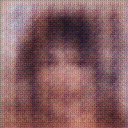
\includegraphics[width=150px]{500_fake_images/samples_5_279.png}%
\caption{A Black And White Photo Of A Cat Looking Out A Window}%
\end{figure}

%
\end{document}